\documentclass[letterpaper,11pt]{exam}
\usepackage{amssymb,amsmath,amsthm,mathtools}
\usepackage{hyperref}
\usepackage{enumitem}
\usepackage{xcolor}
\usepackage{pdfpages}
\usepackage{amsmath}

\usepackage{booktabs}
\usepackage{caption}

\usepackage{pythontex}
\usepackage{listings}
\usepackage{color}
\usepackage{floatflt}
\usepackage{listings}
\usepackage{xcolor}

\setlength{\parskip}{1em}  % Space between paragraphs

\definecolor{dkgreen}{rgb}{0,0.6,0}
\definecolor{gray}{rgb}{0.5,0.5,0.5}
\definecolor{mauve}{rgb}{0.58,0,0.82}

\lstset{frame=tb,
  language=Java,
  aboveskip=3mm,
  belowskip=3mm,
  showstringspaces=false,
  columns=flexible,
  basicstyle={\footnotesize\ttfamily},
  numbers=none,
  numberstyle=\tiny\color{gray},
  keywordstyle=\color{blue},
  commentstyle=\color{dkgreen},
  stringstyle=\color{mauve},
  breaklines=true,
  breakatwhitespace=true,
  tabsize=4,
  frame=none
}

\lstset{
    language=C++,
    basicstyle=\ttfamily\footnotesize,
    keywordstyle=\color{blue},
    commentstyle=\color{gray},
    stringstyle=\color{red},
    % numbers=left,
    % numberstyle=\tiny\color{gray},
    stepnumber=1,
    numbersep=5pt,
    showspaces=false,
    showstringspaces=false,
    breaklines=true,
    frame=none,
    captionpos=b
}

\newcommand{\num}{2}
\newcommand{\topic}{Homework \num, A Simple CUDA Renderer}
\newcommand{\coursenum}{15-418/15-618}
\newcommand{\coursename}{\coursenum\ Parallel Computer Architecture and Programming}
\newcommand{\fullname}{Siqi Guo}
\newcommand{\andrew}{AndrewID: siqiguo}
\setlength{\parindent}{0pt} %don't indent first line of paragraph

\definecolor{lightblue}{rgb}{0.2, 0.7, 1} % Light blue in RGB
\hypersetup{
    colorlinks=true,        % Enable colored links (no boxes)
    linkcolor=lightblue,    % Color of internal links
    citecolor=lightblue,    % Color of citation links
    urlcolor=lightblue      % Color of external hyperlinks
}

\pagestyle{headandfoot}
\runningheader{\fullname}{\coursenum\ \textbf{\topic}}{\andrew}
\firstpagefooter{}{\thepage}{}
\runningfooter{}{\thepage}{}
\extrawidth{.5in}\extraheadheight{-.25in}

\begin{document}

\begin{center}
    {\LARGE\coursename\par}
    {\Large\topic\par}
    \fullname (\andrew) \hfill \today
\end{center}
\printanswers


\begin{questions}
    \question
    \subsection*{CUDA Warm-Up 1: SAXPY (5 pts)}

    To gain a bit of practice writing CUDA programs, the warm-up task is to implement the SAXPY function.

    \begin{enumerate}[label=\roman*.]
        \item \texttt{./saxpy}.
              \begin{lstlisting}[]
---------------------------------------------------------
Found 1 CUDA devices
Device 0: NVIDIA GeForce RTX 2080
    SMs:        46
    Global mem: 7959 MB
    CUDA Cap:   7.5
---------------------------------------------------------
Overall: 74.850 ms              [2.986 GB/s]
    1.006 ms               [222.288 GB/s]
    Total Bytes:240000000Overall: 27.106 ms                [8.246 GB/s]
    1.010 ms               [221.262 GB/s]
    Total Bytes:240000000Overall: 27.158 ms                [8.230 GB/s]
    1.008 ms               [221.678 GB/s]
                    \end{lstlisting}

        \item     \texttt{./cudaSaxpy}.

              \begin{lstlisting}[]
---------------------------------------------------------
Found 1 CUDA devices
Device 0: NVIDIA GeForce RTX 2080
    SMs:        46
    Global mem: 7959 MB
    CUDA Cap:   7.5
---------------------------------------------------------
Kernel: 0.686 ms                [325.663 GB/s]
Overall: 24.608 ms              [9.083 GB/s]
Kernel: 0.685 ms                [326.524 GB/s]
Overall: 25.407 ms              [8.798 GB/s]
Kernel: 0.683 ms                [327.363 GB/s]
Overall: 25.375 ms              [8.808 GB/s]
            \end{lstlisting}


    \end{enumerate}







    % \begin{enumerate}[label=\roman*.]
    % \item This type of problem decomposition is referred as Spatial Decomposition since different spatial regions of the image are computed by different processors.

    %       Note that the processor (eight 3.2 GHz Intel Core i7 processors) only has 8 cores, but each core supports two hyper-threads.
    % \item We partition the image generation work into the appropriate number of horizontal blocks.

    %       \begin{itemize}[label=$\circ$]
    %           \item Speedup is not linear in the number of cores used.
    %           \item The workload is not necessarily evenly distributed among the threads.
    %           \item My measurements show that the elapsed time is not same for each thread, which explains the non-linear speedup due to non-evenly workload.
    %       \end{itemize}

    %       \vspace{0.3cm}      

    % \item Modify the mapping of work to threads to improve speedup to almost 8x on the first two
    %       views of the Mandelbrot set.

    %       To decompose the work into row-wise blocks, we can assign each thread to compute a row of the image.
    %       This way, the workload is more evenly distributed among the threads, we could reach speedup around 7.40x \textasciitilde 7.53x.
    %       For view 1, the speedup from 4 to 8 threads is from 3.81x to 7.47x, but from 8 to 16 threads, the speedup is from 7.47x to 7.40x.
    %       For view 2, the speedup from 4 to 8 threads is from 3.72x to 7.29x, but from 8 to 16 threads, the speedup is from 7.29x to 7.28x.

    %       In my decomposition policy, the scaling behavior are different from 4 to 8 threads and 8 to 16 threads, which indicates 4 to 8 threads speedup is almost linear because all threads have access to independent physical cores. However, 8 to 16 threads speedup is not linear because the threads are sharing the same physical core due to hyper-threading.
    % \end{enumerate}

    \newpage

    \question
    \subsection*{CUDA Warm-Up 2: Parallel Prefix-Sum (10 pts)}
    Find peaks.

    \begin{enumerate}[label=\roman*.]
        \item The implementation of \texttt{cudaScan()} (to get exclusive prefix sum) has been completed and passed the correctness test.

              \begin{lstlisting}[]
siqiguo@ghc28:~/private/15-618-Parallel-Computing/asst2/scan$ ./checker.pl -m scan
Mode: scan
Input: random

--------------
Running tests:
--------------

Element Count: 10000
Correctness passed!
Your Time: 0.173
Target Time: 0.184

Element Count: 100000
Correctness passed!
Your Time: 0.285
Target Time: 0.269

Element Count: 1000000
Correctness passed!
Your Time: 0.755
Target Time: 0.443

Element Count: 2000000
Correctness passed!
Your Time: 1.406
Target Time: 0.842

-------------------------
Scan Score Table:
-------------------------
-------------------------------------------------------------------------
| Element Count   | Target Time     | Your Time       | Score           |
-------------------------------------------------------------------------
| 10000           | 0.184           | 0.173           | 1.25            |
| 100000          | 0.269           | 0.285           | 1.25            |
| 1000000         | 0.443           | 0.755           | 0.880132450331126 |
| 2000000         | 0.842           | 1.406           | 0.898293029871977 |
-------------------------------------------------------------------------
|                                   | Total score:    | 4.2784254802031/5 |
-------------------------------------------------------------------------
                \end{lstlisting}

              \newpage
        \item The implementation of \texttt{find\_peaks()} (to get exclusive prefix sum) has been completed and passed the correctness test.

              \begin{lstlisting}[]
siqiguo@ghc28:~/private/15-618-Parallel-Computing/asst2/scan$ ./checker.pl -m find_peaks
Mode: find_peaks
Input: random

--------------
Running tests:
--------------

Element Count: 10000
Correctness passed!
Your Time: 0.203
Target Time: 0.209

Element Count: 100000
Correctness passed!
Your Time: 0.309
Target Time: 0.299

Element Count: 1000000
Correctness passed!
Your Time: 1.049
Target Time: 0.551

Element Count: 2000000
Correctness passed!
Your Time: 1.848
Target Time: 1.064

-------------------------
Find_peaks Score Table:
-------------------------
-------------------------------------------------------------------------
| Element Count   | Target Time     | Your Time       | Score           |
-------------------------------------------------------------------------
| 10000           | 0.209           | 0.203           | 1.25            |
| 100000          | 0.299           | 0.309           | 1.25            |
| 1000000         | 0.551           | 1.049           | 0.78789323164919 |
| 2000000         | 1.064           | 1.848           | 0.863636363636364 |
-------------------------------------------------------------------------
|                                   | Total score:    | 4.15152959528555/5 |
-------------------------------------------------------------------------
                    \end{lstlisting}
              % \item The implementation of \texttt{clampedExpVector()} should work with any combination of input
              %       array size N and vector width W.
              % \item Run \texttt{./vrun -s 10000} and sweep the vector width over the values {2, 4, 8, 16, 32}.
              %       Record the resulting vector utilization.

              %       \begin{table}[ht]
              %           \centering
              %           \scriptsize
              %           \begin{tabular}{|c|c|c|c|c|c|}
              %               \hline
              %               VECTOR\_WIDTH W           & 2            & 4            & 8            & 16           & 32           \\ \hline
              %               Total Vector Instructions & 276613       & 141698       & 71238        & 35628        & 17787        \\ \hline
              %               Vector Utilization        & 89.066132 \% & 88.370866 \% & 88.216787 \% & 88.211344 \% & 88.212072 \% \\ \hline
              %           \end{tabular}
              %           \caption{Vector Utilization for Different Vector Widths}
              %       \end{table}

              %       The vector utilization decreases as W increases a bit, but the difference is not significant. The degree of sensitivity the utilization has on the vector width is not very high. \\
              %       The higher W is, the more vector instructions are executed.

              % \item \texttt{arraySumVector()} has been implemented, and the results passed the correctness test as follows.

              %       \includegraphics*[width=0.65\textwidth]{./prog2\_vecintrin/arraySumVector.jpg}
    \end{enumerate}



    \newpage

    \question
    \subsection*{A Simple Circle Renderer (85 pts)}

    An implementation of a renderer that draws colored circles.

    \begin{enumerate}[label=\roman*.]
        \item First, given starter code.
              \begin{figure}[h]
                  \begin{minipage}{0.45\textwidth}
                      \centering
                      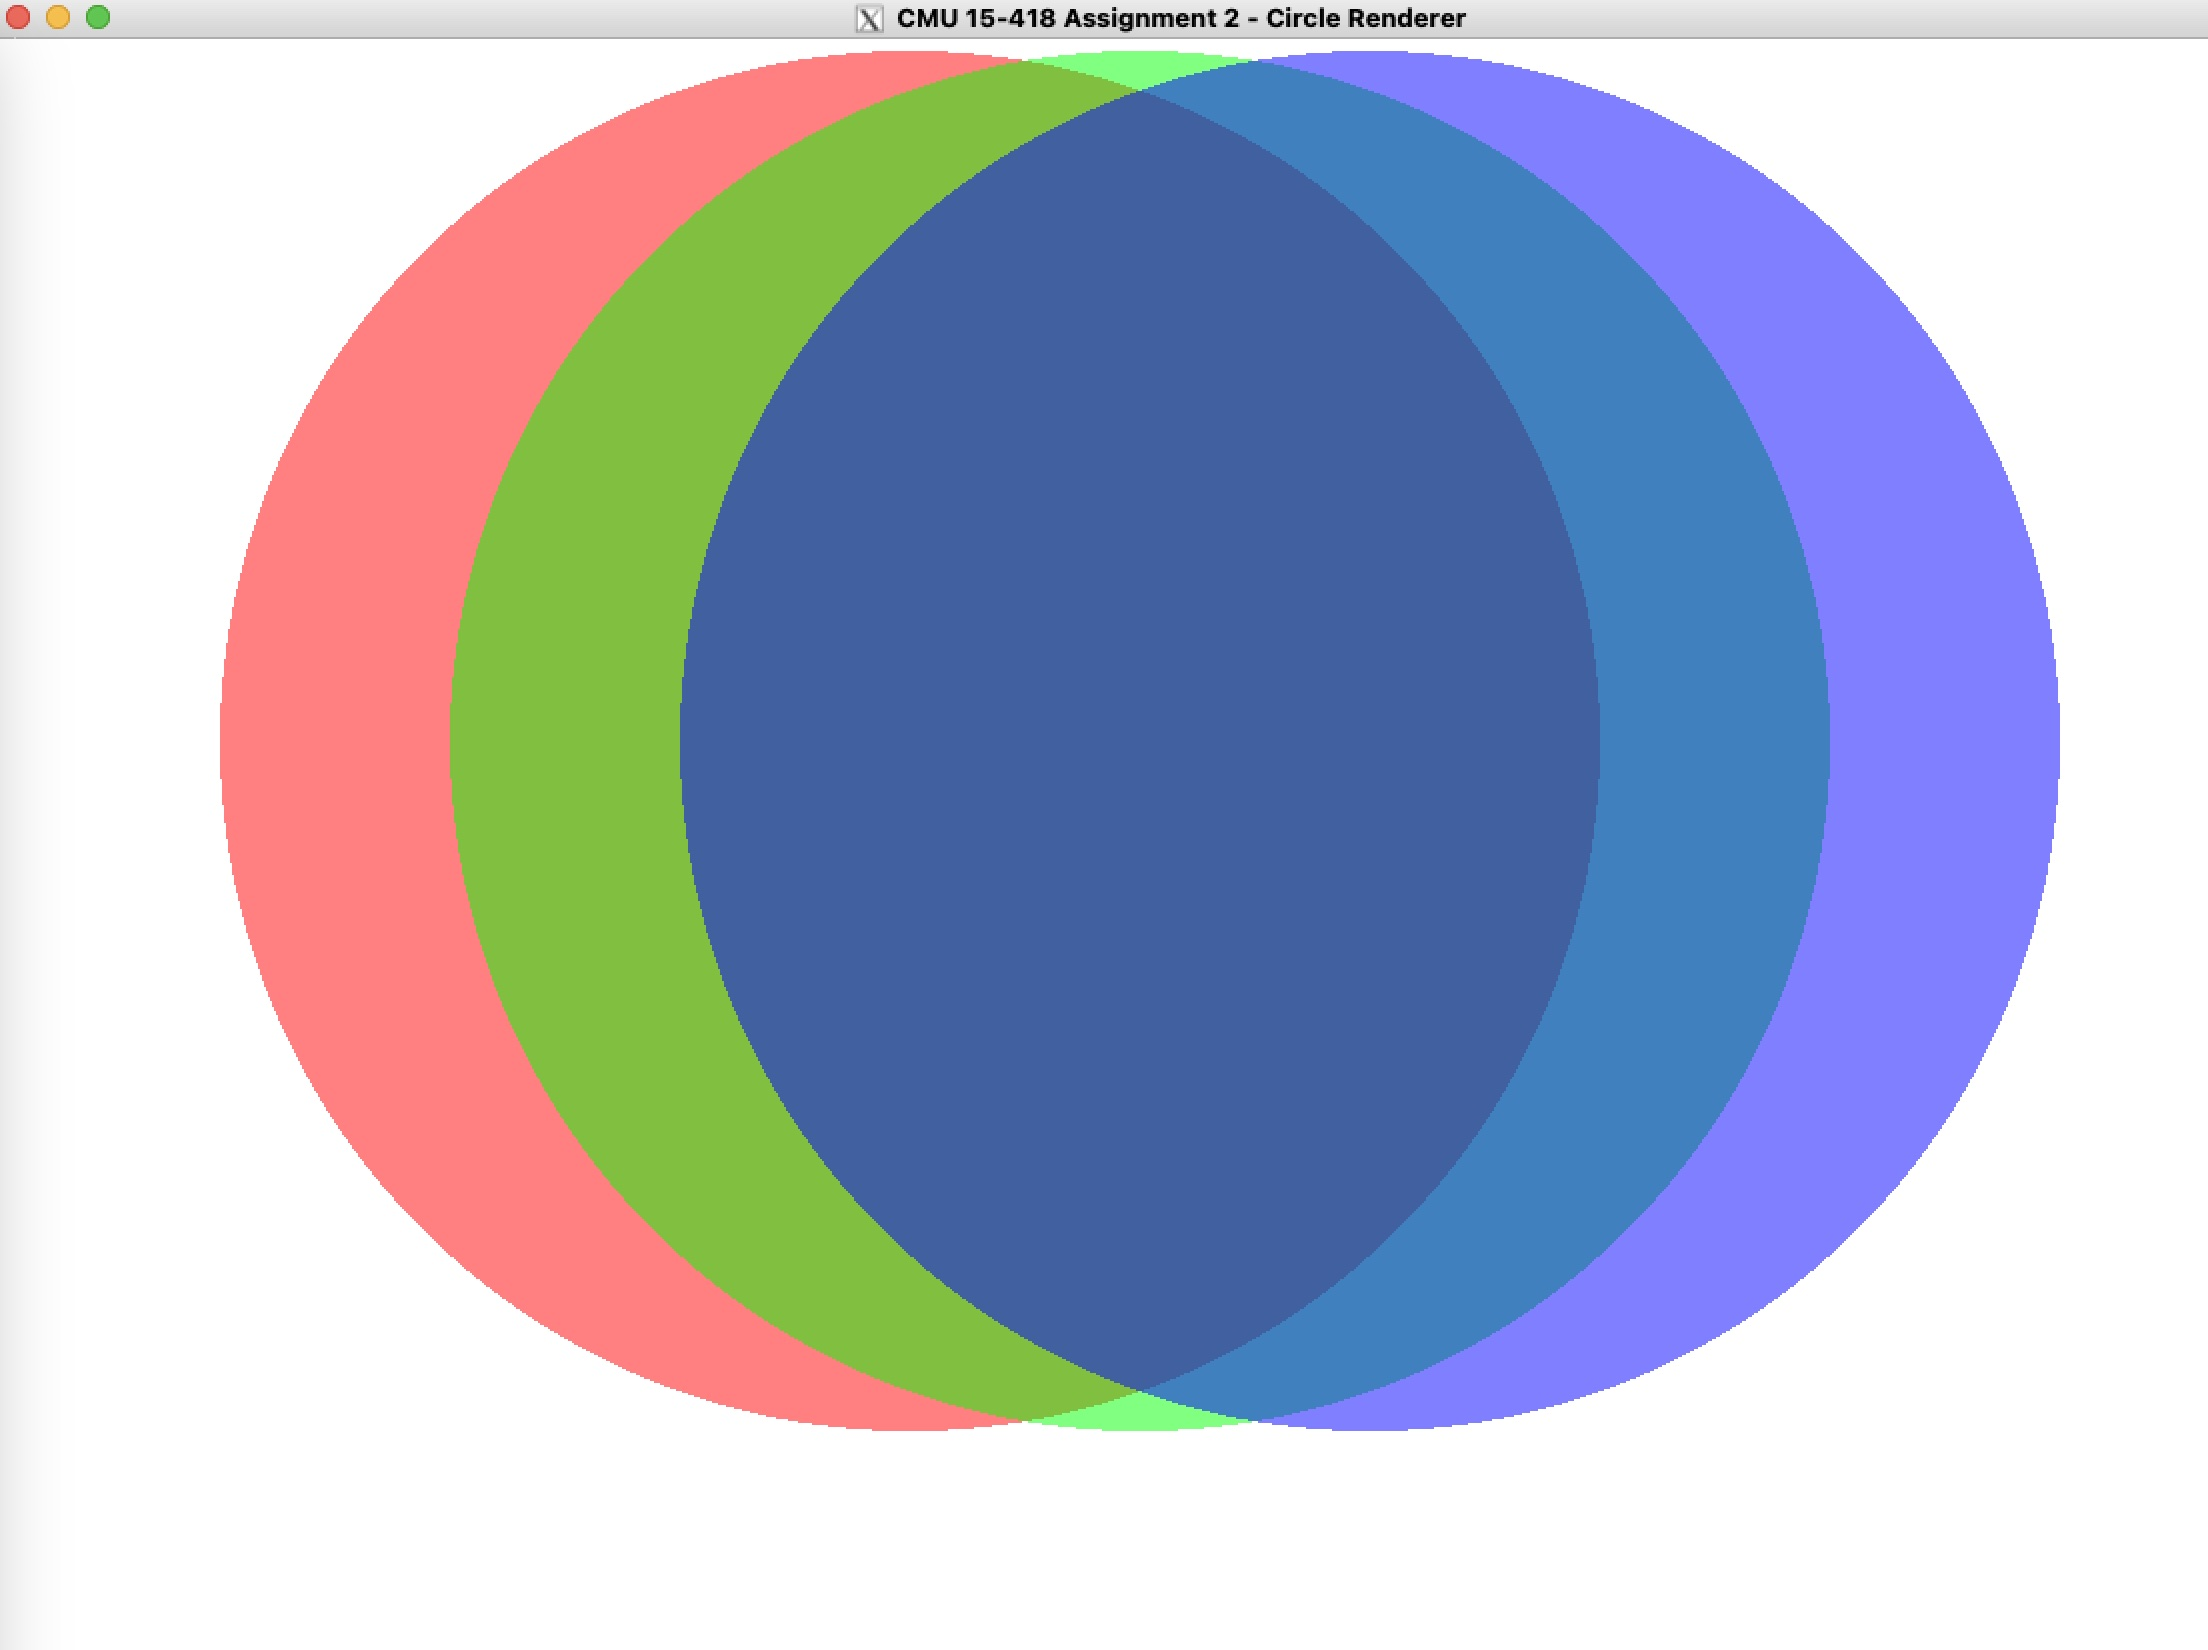
\includegraphics[width=\textwidth]{img/render_rgb.jpg}
                      \label{fig:question3b}
                      \caption{\texttt{./render rgb}}
                  \end{minipage}
                  \hspace{1cm}
                  \begin{minipage}{0.45\textwidth}
                      \centering
                      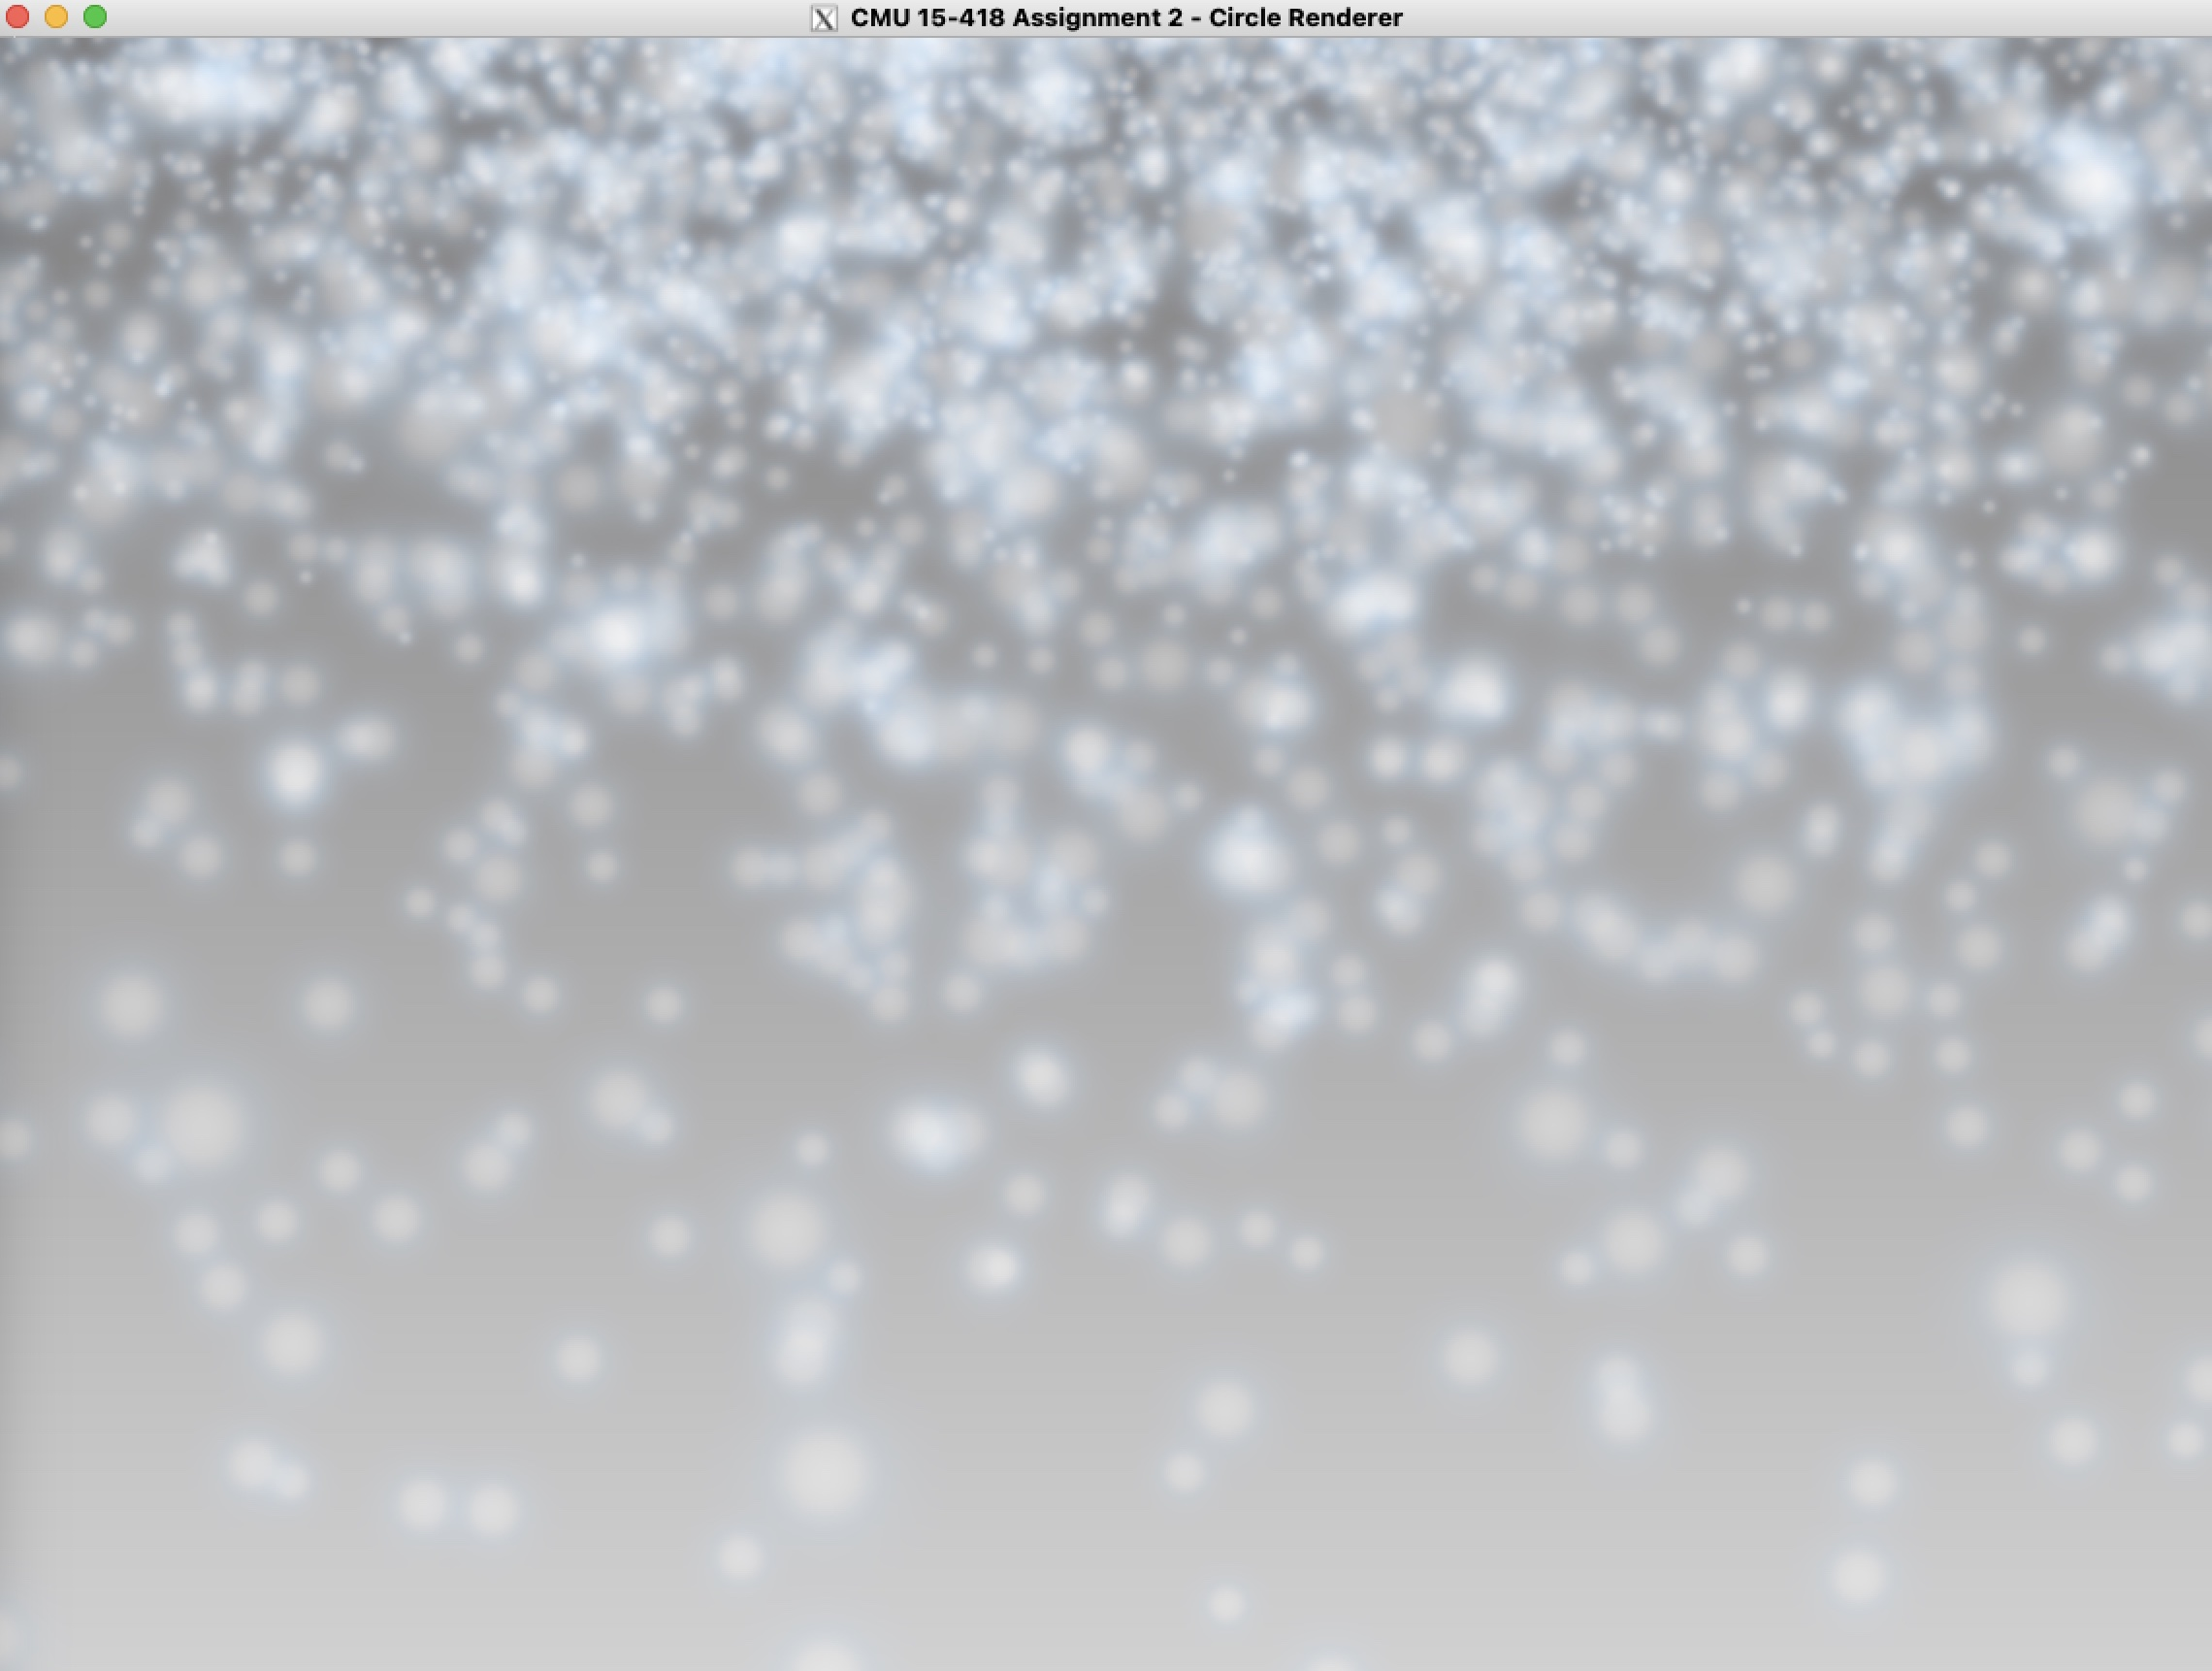
\includegraphics[width=\textwidth]{img/render_snow.jpg}
                      \label{fig:question3b}
                      \caption{\texttt{./render snow}}
                  \end{minipage}
                  %   \hspace{-0.5cm}
                  %   \begin{minipage}{0.5\textwidth}
                  %   \end{minipage}
              \end{figure}

              Machine Info:

              \begin{lstlisting}[]
---------------------------------------------------------
Found 1 CUDA devices
Device 0: NVIDIA GeForce RTX 2080
    SMs:        46
    Global mem: 7959 MB
    CUDA Cap:   7.5
---------------------------------------------------------
              \end{lstlisting}
              \newpage
              Run on starter code.
              \begin{lstlisting}[]
siqiguo@ghc28:~/private/15-618-Parallel-Computing/asst2/render$ make check
mkdir -p objs/
g++ -m64 -O3 -Wall -g -o render objs/main.o objs/display.o objs/benchmark.o objs/refRenderer.o objs/cudaRenderer.o objs/noise.o objs/ppm.o objs/sceneLoader.o -L/usr/local/cuda-11.7/lib64/ -lcudart -lGL -lglut -lcudart 
./checker.pl
Smartmatch is experimental at ./checker.pl line 75.

--------------
Running tests on ghc28.ghc.andrew.cmu.edu, size = 1150, mode = cuda
--------------

Scene : rgb
Correctness failed ... Check ./logs/correctness_rgb.log
Your time : 97.6092
Target Time: 0.1912

Scene : rgby
Correctness failed ... Check ./logs/correctness_rgby.log

Scene : rand10k
Correctness failed ... Check ./logs/correctness_rand10k.log
Your time : 22.5087
Target Time: 1.9674

Scene : rand100k
Correctness failed ... Check ./logs/correctness_rand100k.log
Your time : 502.5219
Target Time: 18.5692

Scene : biglittle
Correctness failed ... Check ./logs/correctness_biglittle.log
Your time : 283.4214
Target Time: 14.2726

Scene : littlebig
Correctness failed ... Check ./logs/correctness_littlebig.log

Scene : pattern
Correctness failed ... Check ./logs/correctness_pattern.log
Your time : 2.8770
Target Time: 0.2756

Scene : bouncingballs
Correctness passed!

Scene : hypnosis
Correctness passed!

Scene : fireworks
Correctness failed ... Check ./logs/correctness_fireworks.log

Scene : snow
Correctness passed!

Scene : snowsingle
Correctness passed!
Your time : 0.0669
Target Time: 0.1779

------------
Score table:
------------
-------------------------------------------------------------------------
| Scene Name      | Target Time     | Your Time       | Score           |
-------------------------------------------------------------------------
| rgb             | 0.1912          | 97.6092 (F)     | 0               |
| rand10k         | 1.9674          | 22.5087 (F)     | 0               |
| rand100k        | 18.5692         | 502.5219 (F)    | 0               |
| pattern         | 0.2756          | 2.8770 (F)      | 0               |
| snowsingle      | 0.1779          | 0.0669          | 12              |
| biglittle       | 14.2726         | 283.4214 (F)    | 0               |
-------------------------------------------------------------------------
|                                   | Total score:    | 12/72           |
-------------------------------------------------------------------------
            \end{lstlisting}


        \item Implementing the CUDA render.

              \begin{itemize}
                  \item First, the render does not meet the atomicity and ordering requirements as it assign the work of rendering each circle to a single thread.
                        The threads are not synchronized, and the result is not deterministic.
                        For each pixel, the thread working on it might not be in the same order as it should be (the circle order provided by the circleIndex).

                        Then, it came to my mind that I should deal with each pixel independently with its required order.
                        Distribute the work of rendering each circle to the threads, then maintain an array to store the order of circles on each pixel.
                        The second step is to distribute the work of each pixel to the threads with the order I have saved.

                        This method works but is not efficient as in the first step we cannot fully utilize the GPU parallelism and the order storage will cause out of memory if the image is too large. Result is as follows.

                        \begin{lstlisting}
siqiguo@ghc28:~/private/15-618-Parallel-Computing/asst2/render$ make check
mkdir -p objs/
g++ -m64 -O3 -Wall -g -o render objs/main.o objs/display.o objs/benchmark.o objs/refRenderer.o objs/cudaRenderer.o objs/noise.o objs/ppm.o objs/sceneLoader.o -L/usr/local/cuda-11.7/lib64/ -lcudart -lGL -lglut -lcudart 
./checker.pl
Smartmatch is experimental at ./checker.pl line 75.

--------------
Running tests on ghc28.ghc.andrew.cmu.edu, size = 1150, mode = cuda
--------------

Scene : rgb
Correctness passed!
Your time : 264.9940
Target Time: 0.2034

Scene : rgby
Correctness passed!

Scene : rand10k
Correctness failed ... Check ./logs/correctness_rand10k.log
Your time : 34.1058
Target Time: 1.9736

Scene : rand100k
Correctness failed ... Check ./logs/correctness_rand100k.log
Your time : 286.9967
Target Time: 18.6039

Scene : biglittle
Correctness failed ... Check ./logs/correctness_biglittle.log
Your time : 289.9027
Target Time: 14.3019

Scene : littlebig
Correctness failed ... Check ./logs/correctness_littlebig.log

Scene : pattern
Correctness passed!
Your time : 380.7105
Target Time: 0.2827

Scene : bouncingballs
Correctness passed!

Scene : hypnosis
Correctness passed!

Scene : fireworks
Correctness passed!

Scene : snow
Correctness passed!

Scene : snowsingle
Correctness passed!
Your time : 3.3260
Target Time: 0.1975

------------
Score table:
------------
-------------------------------------------------------------------------
| Scene Name      | Target Time     | Your Time       | Score           |
-------------------------------------------------------------------------
| rgb             | 0.2034          | 264.9940        | 2               |
| rand10k         | 1.9736          | 34.1058 (F)     | 0               |
| rand100k        | 18.6039         | 286.9967 (F)    | 0               |
| pattern         | 0.2827          | 380.7105        | 2               |
| snowsingle      | 0.1975          | 3.3260          | 2               |
| biglittle       | 14.3019         | 289.9027 (F)    | 0               |
-------------------------------------------------------------------------
|                                   | Total score:    | 6/72            |
-------------------------------------------------------------------------
                  \end{lstlisting}
                        \newpage
                  \item Next, optimize this method with the similar idea. Try to rely on the GPU thread parallelism to accelerate the computation. \\

                        I gained some hints from AI, that I should partition the work of rendering the circles into some subsets of the circles and process them in batches. \\

                        The key idea is to enable as more threads as possible to work. At the very end, each pixel should be processed by one thread.
                        These threads should be assigned the ordering work (store circle index into thread-own buffer) evenly. \\

                        In another view, the image is divided into blocks (corresponding to the GPU blocks), and each block can be processed by a thread block.
                        Each thread in this block is just responsible for a subset of circles to make circle ordering work efficient.
                        The order (circle index) stored in the thread-scope buffer will be merged to the block-scope buffer to make sure later each thread on each pixel can access to all circles in its lifespan. \\

                        \begin{lstlisting}
siqiguo@ghc28:~/private/15-618-Parallel-Computing/asst2/render$ make check
mkdir -p objs/
g++ -m64 -O3 -Wall -g -o render objs/main.o objs/display.o objs/benchmark.o objs/refRenderer.o objs/cudaRenderer.o objs/noise.o objs/ppm.o objs/sceneLoader.o -L/usr/local/cuda-11.7/lib64/ -lcudart -lGL -lglut -lcudart 
./checker.pl
Smartmatch is experimental at ./checker.pl line 75.

--------------
Running tests on ghc28.ghc.andrew.cmu.edu, size = 1024, mode = cuda
--------------

Scene : rgb
Correctness passed!
Your time : 0.1423
Target Time: 0.1523

Scene : rgby
Correctness passed!

Scene : rand10k
Correctness passed!
Your time : 3.7000
Target Time: 1.6040

Scene : rand100k
Correctness passed!
Your time : 34.4337
Target Time: 15.1970

Scene : biglittle
Correctness passed!
Your time : 20.0479
Target Time: 11.4324

Scene : littlebig
Correctness passed!

Scene : pattern
Correctness passed!
Your time : 0.2291
Target Time: 0.2299

Scene : bouncingballs
Correctness passed!

Scene : hypnosis
Correctness passed!

Scene : fireworks
Correctness passed!

Scene : snow
Correctness passed!

Scene : snowsingle
Correctness passed!
Your time : 0.1283
Target Time: 0.1451

------------
Score table:
------------
-------------------------------------------------------------------------
| Scene Name      | Target Time     | Your Time       | Score           |
-------------------------------------------------------------------------
| rgb             | 0.1523          | 0.1423          | 12              |
| rand10k         | 1.6040          | 3.7000          | 7               |
| rand100k        | 15.1970         | 34.4337         | 7               |
| pattern         | 0.2299          | 0.2291          | 12              |
| snowsingle      | 0.1451          | 0.1283          | 12              |
| biglittle       | 11.4324         | 20.0479         | 8               |
-------------------------------------------------------------------------
|                                   | Total score:    | 58/72           |
-------------------------------------------------------------------------
                        \end{lstlisting}

                        More details about the implementation and optimization are in the code comments.
              \end{itemize}

    \end{enumerate}





    \newpage

    % \question
    % \subsection*{Problem 4: Iterative Square Root (10 points)}

    % \begin{enumerate}[label=\roman*.]
    %     \item The sqrt program has been built and run. The speedup due to SIMD (no
    %           tasks) parallelization is 4.77x. The speedup due to multi-core parallelization
    %           is 34.69x.

    %     \item The speedup under different scenarios is as follows.

    %           \begin{table}[ht]
    %               \centering
    %               \scriptsize
    %               \begin{tabular}{|c|c|c|c|}
    %                   \hline
    %                   Case               & Random & initGood & initBad \\ \hline
    %                   SIMD Speedup       & 4.77x  & 6.88x    & 0.95x   \\ \hline
    %                   Multi-Core Speedup & 34.68x & 50.16x   & 6.89x   \\ \hline
    %               \end{tabular}
    %               \caption{Speedup under Different Scenarios}
    %           \end{table}

    %           The \texttt{initGood()} change the value to 2.999. The initialized value of 2.999 could result in the maximum
    %           iteration, and accelerate the paralleled computation to the largest extent. This
    %           modification improves both SIMD and multi-core speedup.

    %           The \texttt{initBad()} change the value to 1.0. The value around 1.0 results in the minimum iteration and the
    %           least absolute computation time. There is not much time to decrease with
    %           parallelism. This modification decreases SIMD and multi-core speedup.

    %           %   \includegraphics*[width=0.65\textwidth]{./prog4\_isqrt/output\_log/speedup_vs_thread_count.png}
    % \end{enumerate}

    % \newpage

    % \question

    % \subsection*{Problem 5: BLAS saxpy (10 points)}

    % The saxpy routine in the BLAS (Basic Linear Algebra Subproblems) library that is
    % widely used (and heavily optimized) on many systems.

    % The \textbf{saxpy} function computes the operation:
    % $\mathbf{r} = a \mathbf{x} + \mathbf{y}$
    % where $a$ is a scalar, and $\mathbf{r}, \mathbf{x}, \mathbf{y}$ are vectors of size $N$ containing single-precision floating-point values.
    % The term \textbf{saxpy} is an acronym for \textbf{"single-precision a x plus y"}.

    % \begin{enumerate}[label=\roman*.]
    %     \item The speedup due to SIMD parallelization is 1x. The speedup from ISPC with tasks is 1.03x.

    %           \captionsetup{font=small, labelfont=bf}
    %           \begin{table}[h!]
    %               \centering
    %               \caption{SAXPY Performance Comparison}
    %               \begin{tabular}{@{}lccc@{}}
    %                   \toprule
    %                   \textbf{Method} & \textbf{Time (ms)} & \textbf{Bandwidth (GB/s)} & \textbf{GFLOPS} \\
    %                   \midrule
    %                   SAXPY Serial    & 11.238             & 26.520                    & 1.780           \\
    %                   SAXPY Streaming & 11.238             & 26.520                    & 1.780           \\
    %                   SAXPY ISPC      & 11.246             & 26.500                    & 1.778           \\
    %                   SAXPY Task ISPC & 10.920             & 27.291                    & 1.831           \\
    %                   \midrule
    %                   \multicolumn{4}{l}{(1.00x speedup from streaming)}                                 \\
    %                   \multicolumn{4}{l}{(1.00x speedup from ISPC)}                                      \\
    %                   \multicolumn{4}{l}{(1.03x speedup from task ISPC)}                                 \\
    %                   \bottomrule
    %               \end{tabular}
    %               \label{tab:saxpy-performance}
    %           \end{table}


    %           I do not think we could achieve linear speedup as the memory bandwidth could be the bottleneck.

    %     \item One value is loaded from vector x \texttt{(N x sizeof(float))}. One value is loaded from vector y \texttt{(N x sizeof(float))}.
    %           One value is written to the result vector  r \texttt{(N x sizeof(float))}.
    %           However, result should be stored in the cache, thus a cache miss will lead to 2 N (read from memory to cache, then back to memory).

    %     \item In addition to the memory bandwidth, the performance of SAXPY might be also limited by poor cache utilization, high cache misses, low pre-fetching efficiency, and the latency of FP operations or DRAM.
    %     \item Improve the performance of saxpy by reducing the memory requirement (modify \texttt{saxpyStreaming()}).
    %           \captionsetup{font=small, labelfont=bf}
    %           \begin{table}[h!]
    %               \centering
    %               \caption{SAXPY Performance Comparison After Streaming}
    %               \begin{tabular}{@{}lccc@{}}
    %                   \toprule
    %                   \textbf{Method} & \textbf{Time (ms)} & \textbf{Bandwidth (GB/s)} & \textbf{GFLOPS} \\
    %                   \midrule
    %                   SAXPY Serial    & 11.280             & 26.421                    & 1.773           \\
    %                   SAXPY Streaming & 8.209              & 36.302                    & 2.436           \\
    %                   SAXPY ISPC      & 11.122             & 26.797                    & 1.798           \\
    %                   SAXPY Task ISPC & 10.900             & 27.342                    & 1.835           \\
    %                   \midrule
    %                   \multicolumn{4}{l}{(1.37x speedup from streaming)}                                 \\
    %                   \multicolumn{4}{l}{(1.01x speedup from ISPC)}                                      \\
    %                   \multicolumn{4}{l}{(1.03x speedup from task ISPC)}                                 \\
    %                   \bottomrule
    %               \end{tabular}
    %               \label{tab:saxpy_comparison}
    %           \end{table}



    % \end{enumerate}

    % Overall, the cache does matter in this problem.

    % \begin{figure}[h]
    %     \begin{minipage}{0.5\textwidth}
    %         \centering
    %         \includegraphics[width=\textwidth]{./hw3_code/plots/question_3a.png}
    %         \label{fig:question3b}
    %     \end{minipage}
    %     \hspace{-0.5cm}
    %     \begin{minipage}{0.5\textwidth}
    %         From the plot, increasing the fraction of clients sampled per round increases the global model's convergence speed and enhances the accuracy with more representative local updates.

    %         However, given the IID data distribution, the performance of the model will not be significantly affected by increasing the fraction of clients sampled per round, compared to the non-IID case.
    %     \end{minipage}
    % \end{figure}

\end{questions}

\end{document}